\documentclass[10pt]{article}
\textwidth 16.5cm
\textheight 23.5cm
\oddsidemargin 0pt
\topmargin -2cm
% \usepackage{epsf}

% Writing maths
\usepackage{
    amsmath, % aligns, equations, etc.
    amsfonts, % blackboard bold, etc.
    bbm, % blackboard bold for numbers.
}

% Figures
\usepackage{graphicx}

% References
\usepackage{hyperref}

% References 
\usepackage[numbers]{natbib}
\bibliographystyle{natbib}
% \setcitestyle{authoryear, open={(},close={)}}

% Inline comments from Jacob and Bella
\usepackage{xcolor}
\usepackage[draft,inline,nomargin,index]{fixme}
\fxsetup{theme=color,mode=multiuser}
\FXRegisterAuthor{jb}{ajb}{\color{blue} JB}
\FXRegisterAuthor{bd}{abd}{\color{red} BD}

\title{Simulations of Immigration Queues at Edinburgh Airport: Report}
 \author{Isabella Deutsch, Jacob R. Bradley
 \\ \emph{School of Mathematics, University of Edinburgh}}

\begin{document}
\maketitle

\section{Introduction}

A large number of passengers arriving in Edinburgh Airport need to pass through immigration. This is either conducted at a \textit{desk} staffed with a Border Force Officer or at an automated \textit{eGate}. This does not apply for anyone arriving from the United Kingdom (including Northern Ireland), the Crown Dependencies, and the Republic of Ireland, as there are no routine passport controls between these countries \cite{common_travel_area}.

Only passengers of certain nationality are eligible to use the eGates, as defined below. There are currently 9 desks and 10 eGates in operation at Edinburgh Airport. As the operations at Edinburgh Airports are changing and growing it is vital to assess the potential impact on queuing time at the border. 

\subsection{Problem Statement}
what is the task, summarising the problem, maybe  outline from the document

\subsection{Key Performance Indicators}

Three key performance indicators were identified in the competition brief. We define them as follows.

\begin{itemize}
    \item \textbf{Queue length}: Number of people in the queue at any given point in time. We report the mean, median, 75\% quantile, and maximum. These are calculated both for the total of the immigration queue, as well as the desk and eGate queues separately.
    \item \textbf{Queue time}: Minutes between the arrival at queue and arrival at a desk/eGate for each arriving passenger. We report the mean, median, 75\% quantile, and maximum. These are calculated both for the total of the immigration queue, as well as the desk and eGate queues separately.
    \item \textbf{Overflow}: Proportion of the day for which the overflow and contingency capacity are used.
\end{itemize}

Note that \textit{Queue length} is measured as a function over time, i.e. we record the queue length every second, even if no passengers are arriving. Based on this granular data we then compute average and maxima statistics. The \textit{queue time}, however, is measured for each arriving passenger.


\section{Data}
This section outlines the data used for our analysis. It contains descriptions of both the data provided through the Modelling Competition and additional data we deemed relevant for this project.

\subsection{Provided Information}

We first outline some of the data received through the Modelling Competition. While these represent realistic values, we are aware that they may contain approximations and/or simulated data. Most notably, the arrivals data in Section~\ref{XX} is a fictitious arrivals schedule for five weeks in the future, in namely 2023 to 2027. 

\subsubsection{Operational Data}

\paragraph{Hall Capacity}
The immigration hall at Edinburgh Airport has a \textit{capacity} of $500$ people. Its \textit{overflow} capacity, which can be used without overly impacting other areas of the operation, is a further $150$ people. There is also a \textit{contingency} capacity for additional $600$ people. However, its usage negatively impacts the operations of the airport.

\paragraph{Coached and Contact}
Once the aircraft has reached its parking position there are two ways for passengers to reach the terminal building. \textit{Contact} passengers walk by foot to the immigration queue. \textit{Coached} passengers exit the aircraft via stairs and are then loaded onto busses, which bring them to the terminal building. The percentage of contact passengers lies above 80\% and varies across years.

\paragraph{eGates Eligibility for EUplus}
Passengers of the following nationalities are allowed to use the eGates: EU countries, Australia, Canada, Iceland, Japan, Liechtenstein, New Zealand, Norway, Singapore, South Korea, Switzerland, and the USA. In the following we refer to these countries as \textit{EUplus}. 

\paragraph{Early and Delayed Flights}
In the summer of 2019 only 58\% of flights arrived on time (measured if arrived within 15 minutes of scheduled arrival), 21\% were late, and 21\% were early. 

\subsubsection{Arrivals Data}
As part of the competition we have received fictitious scheduled arrival data for five weeks (each Monday to Sunday) in the future, containg a total of $4,123$ flights. They are outlined in Table~\ref{tab_comdat_overview}.


\begin{table}[!ht]
\caption{Fictitious data sets provided by the modelling competition.}
\label{tab_comdat_overview}
\centering
\begin{tabular}{ccccc}
\hline
\multicolumn{1}{c}{\textbf{Data Set}} & \textbf{Year} & \textbf{Start Date} & \textbf{End Date} & \textbf{Number of Flights} \\ \hline
1  & 2023  & 10/07  & 16/07     & $665$   \\
2  & 2024  & 08/07  & 14/07     & $768$   \\
3  & 2025  & 14/07  & 20/07     & $843$   \\
4  & 2026  & 13/07  & 19/07     & $894$   \\
5  & 2027  & 12/07  & 18/07     & $953$   \\ \hline
\end{tabular}
\end{table}

As these dates lie, in parts quite far, in the future we can confidently assume that these were simulated for the purpose of this competition. The data sets also include the number of passengers on each flight, but there is no information on their nationalities. In addition, there is also no indication of the departing airport for each flight. This is relevant as only passengers arriving from outside the Common Travel Area need to go through the immigration process \cite{common_travel_area}.



\subsection{Additional Information}


\subsubsection{Operational Data}

\paragraph{Aircraft Capacity and Load Factor}
We obtained a data set indicating the maximum number of passengers for each aircraft type \cite{aircraft_capacity}. The average percentage of occupied seat for a given flight ranges from 86\% in 2019 for international flights in the UK \cite{loading_factor_national} to self-reporter 91\% for a budget airline in 2022 \cite{loading_factor_ryanair}. This is called the \textit{load factor}.

\paragraph{Airport Classification}
We assume that the split in passenger nationality depends on the departing airport. We therefore group airports into the following categories: 
\begin{itemize}
    \item \textbf{UKIE}: All airports in the United Kingdom (including Northern Ireland), the Crown Dependencies, and the Republic of Ireland.
    \item \textbf{EUplus hubs}: Hub airports in EUplus. These are XXXXXXX \cite{mega_hubs}.
    \item \textbf{EUplus non-hubs}: Airports, which are not hubs, located in EUplus.
    \item \textbf{Other hubs}: Hub airports outside of EUplus. These are XXXXXXX \cite{mega_hubs}.
    \item \textbf{Other non-hubs}: Airports, which are not hubs, located outside of EUplus.
\end{itemize}

\paragraph{eGate Utilisation}
The UK government's target of eGate usage among those eligible is at 80\%, which was broadly met on a national level in 2019 and the first quarter of 2020. For airports in the North the uptake was consistently lower at around 70\% for the same period \cite{Inspection_eGates}. While there were no publicly available numbers for Edinburgh Airport, Glasgow Airport's uptake of around 60\% can serve as a reference due to proximity, as well as a lower limit, as it reports some of the lowest utilisation of eGates nationwide \cite{Inspection_eGates}. 

\paragraph{Average Queue Time eGates}
The average queue time at eGates at UK airports for the financial years 2017-18, 2018-19, 2019-20 and Q1 2020 was six minutes and one second \cite{Inspection_eGates}. Stansted and Luton reported averages just below the three minute mark. Glasgow Airport's average waiting time at the eGates was over $8.5$ minutes. However, their calculation was based a shorter time period (December 2017, January 2018 and February 2019), and may therefore be unrepresentative \cite{Inspection_eGates}.


\subsubsection{Arrivals Data}
talk about our fancy arrivals data set we have from 2019 and 2022 \\
here quite a few plots might be needed 


\begin{table}[!ht]
\caption{Historic data sets of Edinburgh Airport Arrivals.}
\label{tab_comdat_overview}
\centering
\begin{tabular}{ccccc}
\hline
\multicolumn{1}{c}{\textbf{Data Set}} & \textbf{Year} & \textbf{Start Date} & \textbf{End Date} & \textbf{Number of Flights} \\ \hline
1  & 2019  & 01/01  & 31/12    &  $51,669$  \\
2  & 2022  & 01/01  & 31/12    &  $31,983$  \\
 \hline
\end{tabular}
\end{table}


\section{Passenger Processing Model}

For our analysis we are using a passenger processing model. It provides an overview over the steps an arriving passenger experiences at Edinburgh airport. It lies in the nature of such a model that it is a simplified view of the world, but we are confident that the chosen level of abstraction is nevertheless informative of the real-world processes at the airport. The passenger processing model consist of three steps, which are outline in detail in the subsequent sections.

The three steps divide the passenger epxerience as as follows:
\begin{enumerate}
    \item \textbf{Aircraft}: Aircraft with passengers on board arrive at Edinburgh Airport. The aircraft taxis to its parking position and the doors are opened. \label{step:aircraft}
    \item \textbf{Route}: Passengers make their way from their aircraft to the immigration hall, either by walking to the building (contact) or via a bus (coached). \label{step:route}
    \item \textbf{Immigration}: Passengers queue in the immigration hall and are processed at the boarder, either at a desk by a Border Force Officer or at an automated eGate. \label{step:immigration}
\end{enumerate}

 Figure~\ref{PPM_threesteps} visualises the flow of information from a data perspective. We start with a data set of arriving flights and generate a data set of passengers (\textit{Aircraft} step). In the \textit{Route} step these passengers are then brought from the aircraft to the immigration hall. Finally, in the \textit{Immigration} step they queue up and are subsequently processes at the border.

\begin{figure}[!ht]
    \centering
    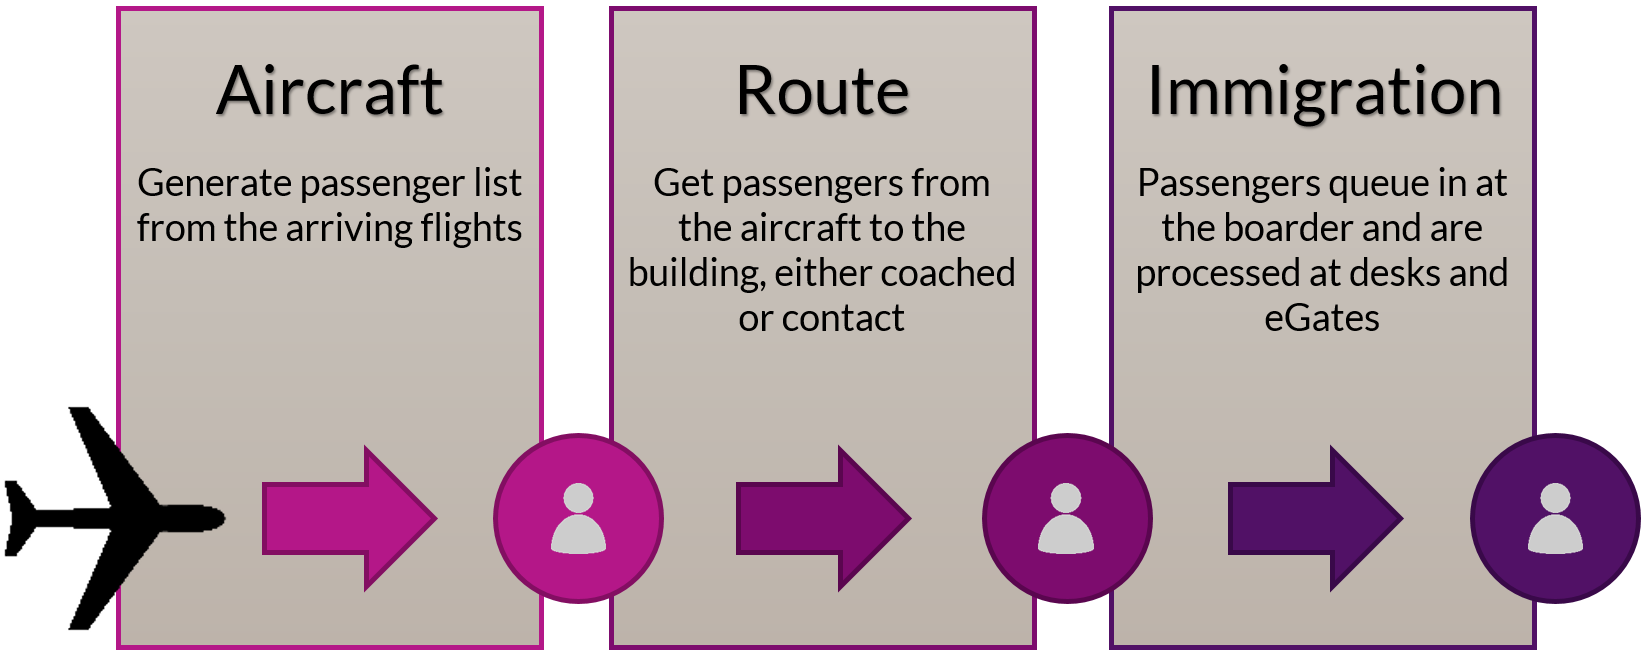
\includegraphics[width=0.7\textwidth]{figures/ThreeSteps.png}
     \caption{Three steps that make up the passenger processing model. } \label{PPM_threesteps}
\end{figure}


\section{Simulation Analysis for Provided Data}

\subsection{Methodology}
We explain how we simulate the airports they came from \\
describe any other simulation input needed, maybe different scenarios \\ 
be clear that this is (almost) just what they asked for  \\ Assumption: provided flights are all/mostly non-UKIE (compare to Noise data set)

\subsection{Results}
include KPIs here, as well as some fancy plots


\section{Simulation Analysis for Additional Data}

\subsection{Methodology}
we take real days and simulate worse (but realistic) days and do the analysis again

\subsection{Results}
include KPIs here, as well as some fancy plots


\section{Robustness Considerations}
relate to service level agreement \\
talk about working eGates/break down of eGates  \\
what if there are more non-UKIE flights 

\section{Discussion}
summary of the project and our approach


\subsection{Recommendation for Total Number of eGates}
we need to put our foot down and come up with a final number

\subsection{Future Work}
all the assumptions we made \\
to include limitations \\
include edge cases, such as all gates closed for high risk flights (see Government doc on eGates) 

\bibliography{report/references.bib}

\end{document}